
%(BEGIN_QUESTION)
% Copyright 2015, Tony R. Kuphaldt, released under the Creative Commons Attribution License (v 1.0)
% This means you may do almost anything with this work of mine, so long as you give me proper credit

A mechanic has an idea for upgrading the electrical system in an automobile originally designed for 6 volt operation.  He wants to upgrade the 6 volt headlights, starter motor, battery, etc, to 12 volts, but wishes to retain the original 6-volt generator and regulator.  Shown here is the original 6-volt electrical system:

$$\includegraphics[width=15.5cm]{i02651x01.eps}$$

The mechanic's plan is to replace all the 6-volt loads with 12-volt loads, and use two 6-volt batteries connected in series, with the original (6-volt) regulator sensing voltage across only one of those batteries:

$$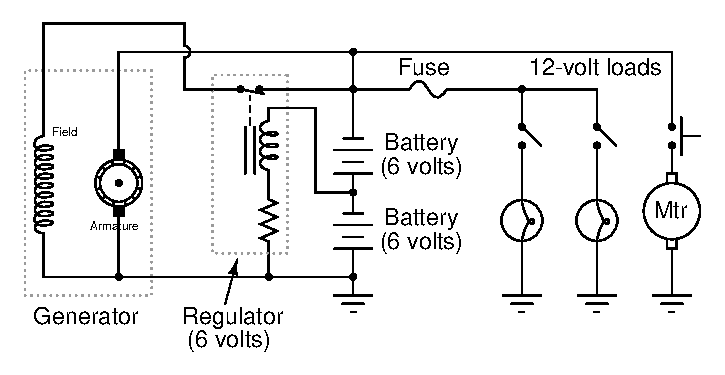
\includegraphics[width=15.5cm]{i02651x02.eps}$$

Explain how this system is supposed to work.  Do you think the mechanic's plan is practical, or are there any problems with it?

\underbar{file i02651}
%(END_QUESTION)





%(BEGIN_ANSWER)

So long as the generator is capable of outputting 12 volts, this system will work!

\vskip 10pt

In this question, we see a foreshadowing of op-amp theory, with the regulator's negative feedback applied to what is essentially a voltage divider (two equal-voltage batteries being charged by the generator).  The regulator circuit senses only 6 volts, but the generator outputs 12 volts.  Fundamentally, the focus of this question is {\it negative feedback} and one of its many practical applications in electrical engineering.

\vskip 10pt

This idea actually came from my father, who did this very thing on an International T-4 bulldozer.  An important difference is that he used a single 12-volt battery rather than two 6-volt batteries, creating a center-tap connection on the 12-volt battery to make it perform as two 6-volt batteries.  To do this, he carefully drilled a hole in the top of the battery to intersect with the lead bus bar between the third and fourth cells, threading a screw into that bus bar as the center-tap terminal.  In fact, the entire motivation for this project was that it was far cheaper for him to get a new 12-volt battery than to buy a new 6-volt battery, and he had plenty of 12-volt electrical accessories (headlights, ignition coils, etc.) to upgrade the bulldozer.

\vskip 10pt

One of the readers of my online textbook wished to do something similar, except his plan was to make the vehicle's original 12-volt system output 24 volts so he could power surplus military accessories.  An important distinction for this fellow's system is that he planned to have more than a few 12-volt loads remaining in the vehicle, such as a 12-volt radio:

$$\includegraphics[width=15.5cm]{i02651x03.eps}$$

As a challenge for your students, ask them how well they think {\it this} system would work.  It is a bit more complex than the system shown in the question, due to the two different load banks.

%(END_ANSWER)





%(BEGIN_NOTES)


%INDEX% Negative feedback, in DC generator voltage regulation system
%INDEX% Voltage regulator, DC generator

%(END_NOTES)


